%%%%%%%%%%%%%%%%%%%%%%%%%%%%%%%%%%%%%%%%%
% Stylish Article
% LaTeX Template
% Version 2.1 (1/10/15)
%
% This template has been downloaded from:
% http://www.LaTeXTemplates.com
%
% Original author:
% Mathias Legrand (legrand.mathias@gmail.com) 
% With extensive modifications by:
% Vel (vel@latextemplates.com)
%
% License:
% CC BY-NC-SA 3.0 (http://creativecommons.org/licenses/by-nc-sa/3.0/)
%
%%%%%%%%%%%%%%%%%%%%%%%%%%%%%%%%%%%%%%%%%

%----------------------------------------------------------------------------------------
%	PACKAGES AND OTHER DOCUMENT CONFIGURATIONS
%----------------------------------------------------------------------------------------

\documentclass[fleqn,10pt]{SelfArx} % Document font size and equations flushed left
\usepackage[english]{babel} % Specify a different language here - english by default

\usepackage{lipsum} % Required to insert dummy text. To be removed otherwise
\usepackage{blindtext}
\usepackage{listings} % Required to include the codes

%----------------------------------------------------------------------------------------
%	COLUMNS
%----------------------------------------------------------------------------------------

\setlength{\columnsep}{0.55cm} % Distance between the two columns of text
\setlength{\fboxrule}{0.75pt} % Width of the border around the abstract

%----------------------------------------------------------------------------------------
%	COLORS
%----------------------------------------------------------------------------------------

\definecolor{color1}{RGB}{0,0,90} % Color of the article title and sections
\definecolor{color2}{RGB}{0,20,20} % Color of the boxes behind the abstract and headings

%----------------------------------------------------------------------------------------
%	HYPERLINKS
%----------------------------------------------------------------------------------------

\usepackage{hyperref} % Required for hyperlinks
\hypersetup{hidelinks,colorlinks,breaklinks=true,urlcolor=color2,citecolor=color1,linkcolor=color1,bookmarksopen=false,pdftitle={Title},pdfauthor={Author}}

%----------------------------------------------------------------------------------------
%	ARTICLE INFORMATION
%----------------------------------------------------------------------------------------

\JournalInfo{Data Mining B565 Fall 2016} % Journal information
\Archive{} % Additional notes (e.g. copyright, DOI, review/research article)

\PaperTitle{Title Here *****} % Article title

\Authors{Ethan Lee\textsuperscript{1}*, Saheli Saha\textsuperscript{1}} % Authors

\affiliation{\textsuperscript{1}\textit{Department of Computer Science, School of Informatics and Computing, Indiana University, Bloomington, IN, USA}} % Author affiliation
\affiliation{*\textbf{Corresponding author}: sasaha@iu.edu} % Corresponding author

\Keywords{***** Keyword1 --- Keyword2 --- Keyword3} % Keywords - if you don't want any simply remove all the text between the curly brackets
\newcommand{\keywordname}{Keywords} % Defines the keywords heading name

%----------------------------------------------------------------------------------------
%	ABSTRACT
%----------------------------------------------------------------------------------------

\Abstract{Abstract here *****}

%----------------------------------------------------------------------------------------

\begin{document}

\flushbottom % Makes all text pages the same height

\maketitle % Print the title and abstract box

\tableofcontents % Print the contents section

\thispagestyle{empty} % Removes page numbering from the first page

%----------------------------------------------------------------------------------------
%	ARTICLE CONTENTS
%----------------------------------------------------------------------------------------

\section*{Introduction} % The \section*{} command stops section numbering

\addcontentsline{toc}{section}{Introduction} % Adds this section to the table of contents

% Intro here *****. Problem in general. Historical context, money - why this is interesting. Should be exciting. Not Kaggle.
% 1 page

With a home being the largest purchase most people will ever make, it is not surprising that housing price prediction is a frequently-studied task. Highly reliable price predictions would bring many economic benefits. Sellers and buyers could both be certain of a fair deal. Realtors could set prices perfectly according to the seller's goals, whether to sell quickly at a low price or more slowly at a somewhat higher price. Tax assessors could give accurate valuations of homes. And perhaps most intriguingly, civic organizations and government officials could run models of the effect of various policies on housing prices, enabling more effective building regulations, zoning laws, and city planning.

Of course there are many barriers to achieving this ideal. Many interacting components affect price, including not just physical features of the home, but buyer demographics, the rental market, land prices, construction costs, the regulatory environment, crime rates, school quality, and proximity to various facilities, to name a few. At present, the most accurate way to determine home value is to sell it. Of course this is not always a desired course of action, and may not even reflect worth accurately. For example, emotions of the buyer and seller can affect sale price, in the form of exhaustion with the buying/selling process, idiosyncratic preferences, or even personal feelings about others involved in the transaction. 

This paper nevertheless explores strategies for making housing price predictions using the Ames, Iowa, U.S.A. data-set. *****

%Ames set is excellent, but still not enough. the attributes in the Ames set capture some of this indirectly, and some not at all. %A single city, so model that works for this market may not work for others anyway

%We do a lot of data cleaning, statistical modeling with *****. Get decent results, and ideas for next steps.

%------------------------------------------------

\section{Background}

In this paper we explore the common method of {\it hedonic regression} in housing price prediction. In this approach, the price of a house is estimated based on a variety of attributes, each assumed to contribute to varying degrees to the true worth. The amount of contribution of each attribute to the price is determined via some form of regression analysis.

Many potential attributes seem rather obvious. For example, square footage should clearly be considered, because homes with greater square footage tend to sell for more. There are many additional attributes of this type representing physical qualities of the house, such as construction material, number of storys, bedrooms, and bathrooms, year constructed, kitchen quality, etc. The Ames dataset considered here includes numerous such attributes as described in more detail below.

A number of researchers, however, have demonstrated the importance and complexity of many other attributes as well -- attributes not directly connected to the physical house itself. For example,  study the influence of transportation and access to facilities. On the one hand, proximity to larger roads means greater potential for noise pollution and traffic, therefore reducing home prices. On the other hand, significant distance from such thoroughfares can mean reduced access to facilities, and therefore reduced home prices for the opposite reason. They show that simplified models of access based on a theoretical central hub are insufficient for accurate price analysis. Furthermore, access is not always desirable, as university and commerce access often leads to higher prices, while K-12 education and industry access often leads to lower prices.

Considering other forms of transportation, proximity to a subway stop can boost home prices in some markets  while proximity to an airport can either increase or decrease home prices depending on the presence of noise pollution . In most transportation modes, the convenience of proximity can also be offset by a reduction in air quality, particularly in areas with higher average incomes .

Broad categories of locations can also greatly influence home prices.  demonstrates the different effects of physical improvements and neighborhood quality in suburban versus urban environments, leading to a recommendation for entirely different price models for the two categories. The number of land-use and building regulations can reduce vacant land values but increase home values  with such regulations being a major factor in high prices in San Francisco  and Manhattan , and in a study of 56 major cities across the United States. Furthermore, not just the immediate regulatory environment but also the number of nearby distinct jurisdictions affect home prices in interacting ways 

Further potential attributes for hedonic regression include the rental market, land prices, and constructions costs  presence of registered sex offenders  and even the education level and age of typical local buyers . The list of potentially relevant attributes in a hedonic regression seems nearly endless, such that even the impressively comprehensive Ames, IA dataset is inadequate for perfect prediction. Since one cannot simply wait for ``better data'', however, we nevertheless proceed in developing a model of housing prices on this dataset.

%------------------------------------------------

\section{Algorithm and Methodology}
\subsection{House Price Prediction}

 \subsubsection{Data Analysis}

The Ames, Iwoa dataset - is the dataset on which we are doing the prediction on. 
It is comprised with eighty features to describe the Houses to be sold. In this Ames Dataset 
all the features are the variables that buyer would like to know before buying any house.
\\ There are fourteen discrete features to describe any particular house. Such as Number of Kitchens, type of bathroom i.e: Half or Full, Type of Street accessed to the property Gravel or Paved. Additionally Garage type or Land-slope types are also provided. 
\\There are twenty features to describe the dimension of the houses. It is  described in detail with the combination of common features like Lot Size, 
Dwelling Size and extraneous features like, Basement's Dimension, Living Area or Porch's dimension.Again these dimensions are divided into categorical data.
\\Large number of categorical data provided to analyze, Twenty Three nominal and twenty three ordinal. These data varies in a large way. One or two features like Street, has two kinds of values- Gravel or Paved. Many attributes like Neighbourhood or Type of Exteriors varies from seventeen to twenty five kind of values.

We have categorised some features depending on the approaches we are using. Such as the features which are describing the quality of the House, (ExterQual, BsmtQual, HeatingQC, KitchenQual, FireplaceQu, GarageQual, PoolQC, Fence) are considered as Ordinal Data, we have ranked those data in a scale of 0 to 10.  


\subsubsection{Data Cleaning}

For the house price prediction this is the main section to work on. After going through the data we realize proper approach to clean the data will give us more accurate results. 
\\For each and every feature we have taken certain approaches to clean that. 

One of the biggest challenge is to converting categorical variables to numerical variables. Although different algorithms are there, we preferred to analyze the nature of the feature and then we started doing engineering on that.

At first we removed all NA values in a meaningful manner.
For example in Alley NA means no Alley so we replaced NA there with No Alley.
We did same with BsmtQual, BsmtCond, BsmtExpo, BsmntFintype1, BsmntFintype2, Fence and SaleCondition.

After transforming the values in order to make it numerical we ranked it in numerical scale. Features like Utilities, HeatingQC, SaleCondition are ranked with o and 1 as they have only two kind of values.

Features like ExterQual, ExterCond or KitchenQual which has five different kind of values has ranked those from one to five. Features which had NA in their value and transformed to zero are ranked from zero to five such as BsmtCond, FireplaceQu.

Features with three different kind of qualities are ranked between zero to three according to their condition. For example OverallCond has one to nine rating. Now I have combined this value in zero to three, from low to high rating respectively.

Features like BsmtFinType1 or BsmtFinType2 which has eight different kind of values are merged into two type of values- zero and one according to their quality condition.

Finally for better result important features like LotFrontage,	LotArea, OverallQual, OverallCond, ExterQual, ExterCond, BsmtCond, GarageQual, GarageCond, KitchenQual, HeatingQC, HeatingQC, MasVnrType, SaleCondition, Reconstruct and ReconstructAfterBuy are calculated as polyvariate values after transforming the NA values to zero.

Finally we used dummy variable algorithm for features like Exterior1st, Exterior2nd, RoofMatl, Condition1, Condition2 and BldgType. 

\subsubsection{Methodology}

After cleaning the data there are several algorithms that we can apply to predict the house price. We were quite sure that simple linear regression was never a good idea to predict accurately. So I started experimenting with different regression techniques. For my cleaned data Lasso regression proved to be the best choice. 

Regression[1] can be defined as a statistical model for prediction, which estimate relationship among variables. It includes techniques like modelling, analyzing, feature selection depending on the dependent and independent variables.

Lasso Regression is one of the regression technique which does both regression and feature selection. Hence, we have not used any other feature selecting algorithm on our clean data. 

\textbf{Lasso Regression} \\ Suppose[2] that we have data $(X^i,y)$, where i = 1,2,....,N and $x^1 = (x_i1,....., x_ip)^T$ are the predictor variables and $y_i$ are the responses. As in the regression set up we assume either the observations are independent or the $y_i s$ are conditionally independent, given the $x_ij s$. We assume that the $x_ij$ are standardized, so that $\sum_i x_ij/N = 0$ $\sum_i x_{ij}^{2}/N = 1$.

Letting $\hat{\beta}$ = $(\hat{\beta}_1,...., \hat{\beta}_p )^T$, the Lasso estimate $(\hat{\alpha}, \hat{\beta})$ is defined by,

$(\hat{\alpha}, \hat{\beta})$ = arg min$\{\sum_{i=1}^{N}(y_i - \alpha - \sum_j \beta_j - x_{ij} )^2\}$ Subject to $\sum_j \mid \beta_j \mid \leq t.$  .... (1)

Here, t $\geq$ 0 is a tuning parameter. Now for all t, solution for $\alpha$ is $\hat{\alpha}$ = $\bar{y}$. We can assume that the loss of generality $\bar{y}$ = 0 and hence omit $\alpha$.

Solution of equation 1 is a quadratic programming problem with linear inequality constraint. The parameter t $\geq$ 0 controls the amount of shrinkage that is applied to the estimates. 

\subsubsection{Implementation}
Lasso regression have powerful statistical and computational advantages and it provides a simplicity and sparsity to the solution. 
I have used to Python clean and predicting the house sale price. 

Python has very useful packages like pandas and numpy for storing and cleaning the data respectively.

For applying the algorithm we have used Sci-kit learn package[3]. It is a free software machine learning library in python which supports classification, regression and clustering algorithms. 
\\We have used Lasso Regression in a following way:-
\\import pandas as pd
\\import numpy as np
\\from sklearn$.$linear\_model import Lasso
\\model\_lasso = Lasso(alpha=5e-4, max\_iter=50000)$.$fit(X\_train, y)
\\coef = pd.Series(model\_lasso.coef\_, index = X\_train\.columns).\\ sort\_values()
\\imp\_coef = pd.concat([coef.head(10), coef$.$tail(10)])
\\Using Sklearn package we are applying Lasso function in our train data first and then this model is predicting house price in from our test data.
\section{Experiments and Results}

\subsection{Experimental Setup}

As part of the data cleaning process first I have used many plotting to understand nature and cleaning method. 
For example I have considered Sale condition as a very important feature for this prediction. So I have done the plotting to understand the co-relation.

\begin{figure}[ht]\centering % Using \begin{figure*} makes the figure take up the entire width of the page
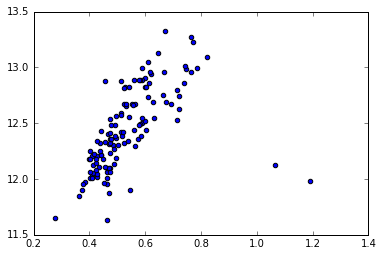
\includegraphics[width=\linewidth]{Figure3}
\caption{Nature of Sale Condition Feature}
\label{fig:Figure3}
\end{figure}

At first I applied dummy variable follwoing that RFE feature selection algorithm to select certain features.  Then we tried to apply different kind of regression algorithms like Linear Regression, Random Forest, Ridge and finally Lasso. Since Lasso has the feature selection ability so we applied Lasso on the cleaned data directly.

while applied Random Forest on the data we got the following graph for error values.

\begin{figure}[ht]\centering % Using \begin{figure*} makes the figure take up the entire width of the page
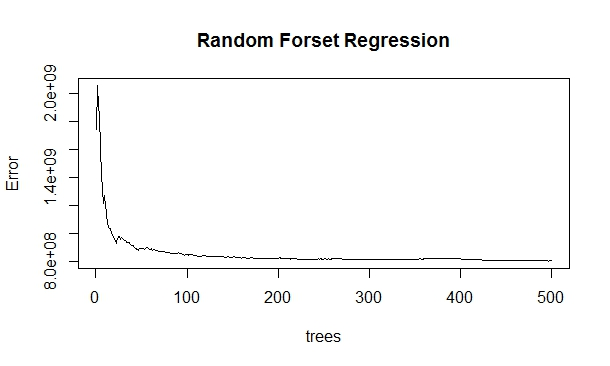
\includegraphics[width=\linewidth]{Figure4}
\caption{Error Rates For Random Forest}
\label{fig:Figure4}
\end{figure}

With this data in Kaggle we got a score of 0.29392.To improve our prediction I tried Ridge and Lasso Algorithm.
After performing Lasso regression we have plotted the co-efficients to understand the nature.

\begin{figure}[ht]\centering % Using \begin{figure*} makes the figure take up the entire width of the page
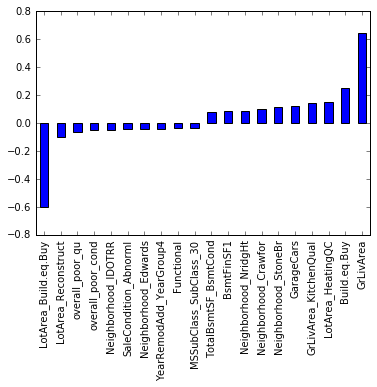
\includegraphics[width=\linewidth]{Figure1}
\caption{Coefficients in the Model}
\label{fig:Figure1}
\end{figure}
We have also done tuning of the parameters in for the algorithm. Ridge and Lasso varies mainly for the $\alpha$ . So, I tried to apply the best fit for $\alpha$.
After tuning $\alpha$ and plotting it I got the following graph.
\begin{figure}[ht]\centering % Using \begin{figure*} makes the figure take up the entire width of the page
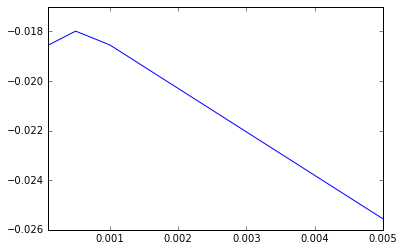
\includegraphics[width=\linewidth]{Figure5}
\caption{Tuning of $\alpha$ For Regression }
\label{fig:Figure5}
\end{figure}

As we can see the formation of co-efficients are giving us a proper linear relation around the regression line. So I considered this model to be best for my data. 

\subsection{Results}

After applying Lasso we got prediction variable with the following visualization:- 
\begin{figure}[ht]\centering % Using \begin{figure*} makes the figure take up the entire width of the page
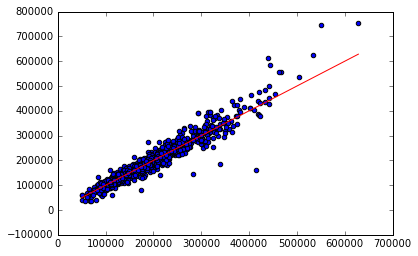
\includegraphics[width=\linewidth]{Figure2}
\caption{Regression Line}
\label{fig:Figure2}
\end{figure}

Applying Lasso we improved our score a lot and now our score is 0.12188.

\subsection{Analysis}

interpretation

Reflect on what happened
why important
objective and subjective


\section{Summary and Conclusions}

3-4 sentence executive summary
what's the bottom line

%------------------------------------------------
\phantomsection
\section*{Acknowledgments} % The \section*{} command stops section numbering

Here*****

\addcontentsline{toc}{section}{Acknowledgments} % Adds this section to the table of contents

%----------------------------------------------------------------------------------------
%	REFERENCE LIST
%----------------------------------------------------------------------------------------
\phantomsection
\bibliographystyle{unsrt}
\bibliography{housingBib}

%----------------------------------------------------------------------------------------

\end{document}